\begin{figure}[htbp]
    \centering{}
    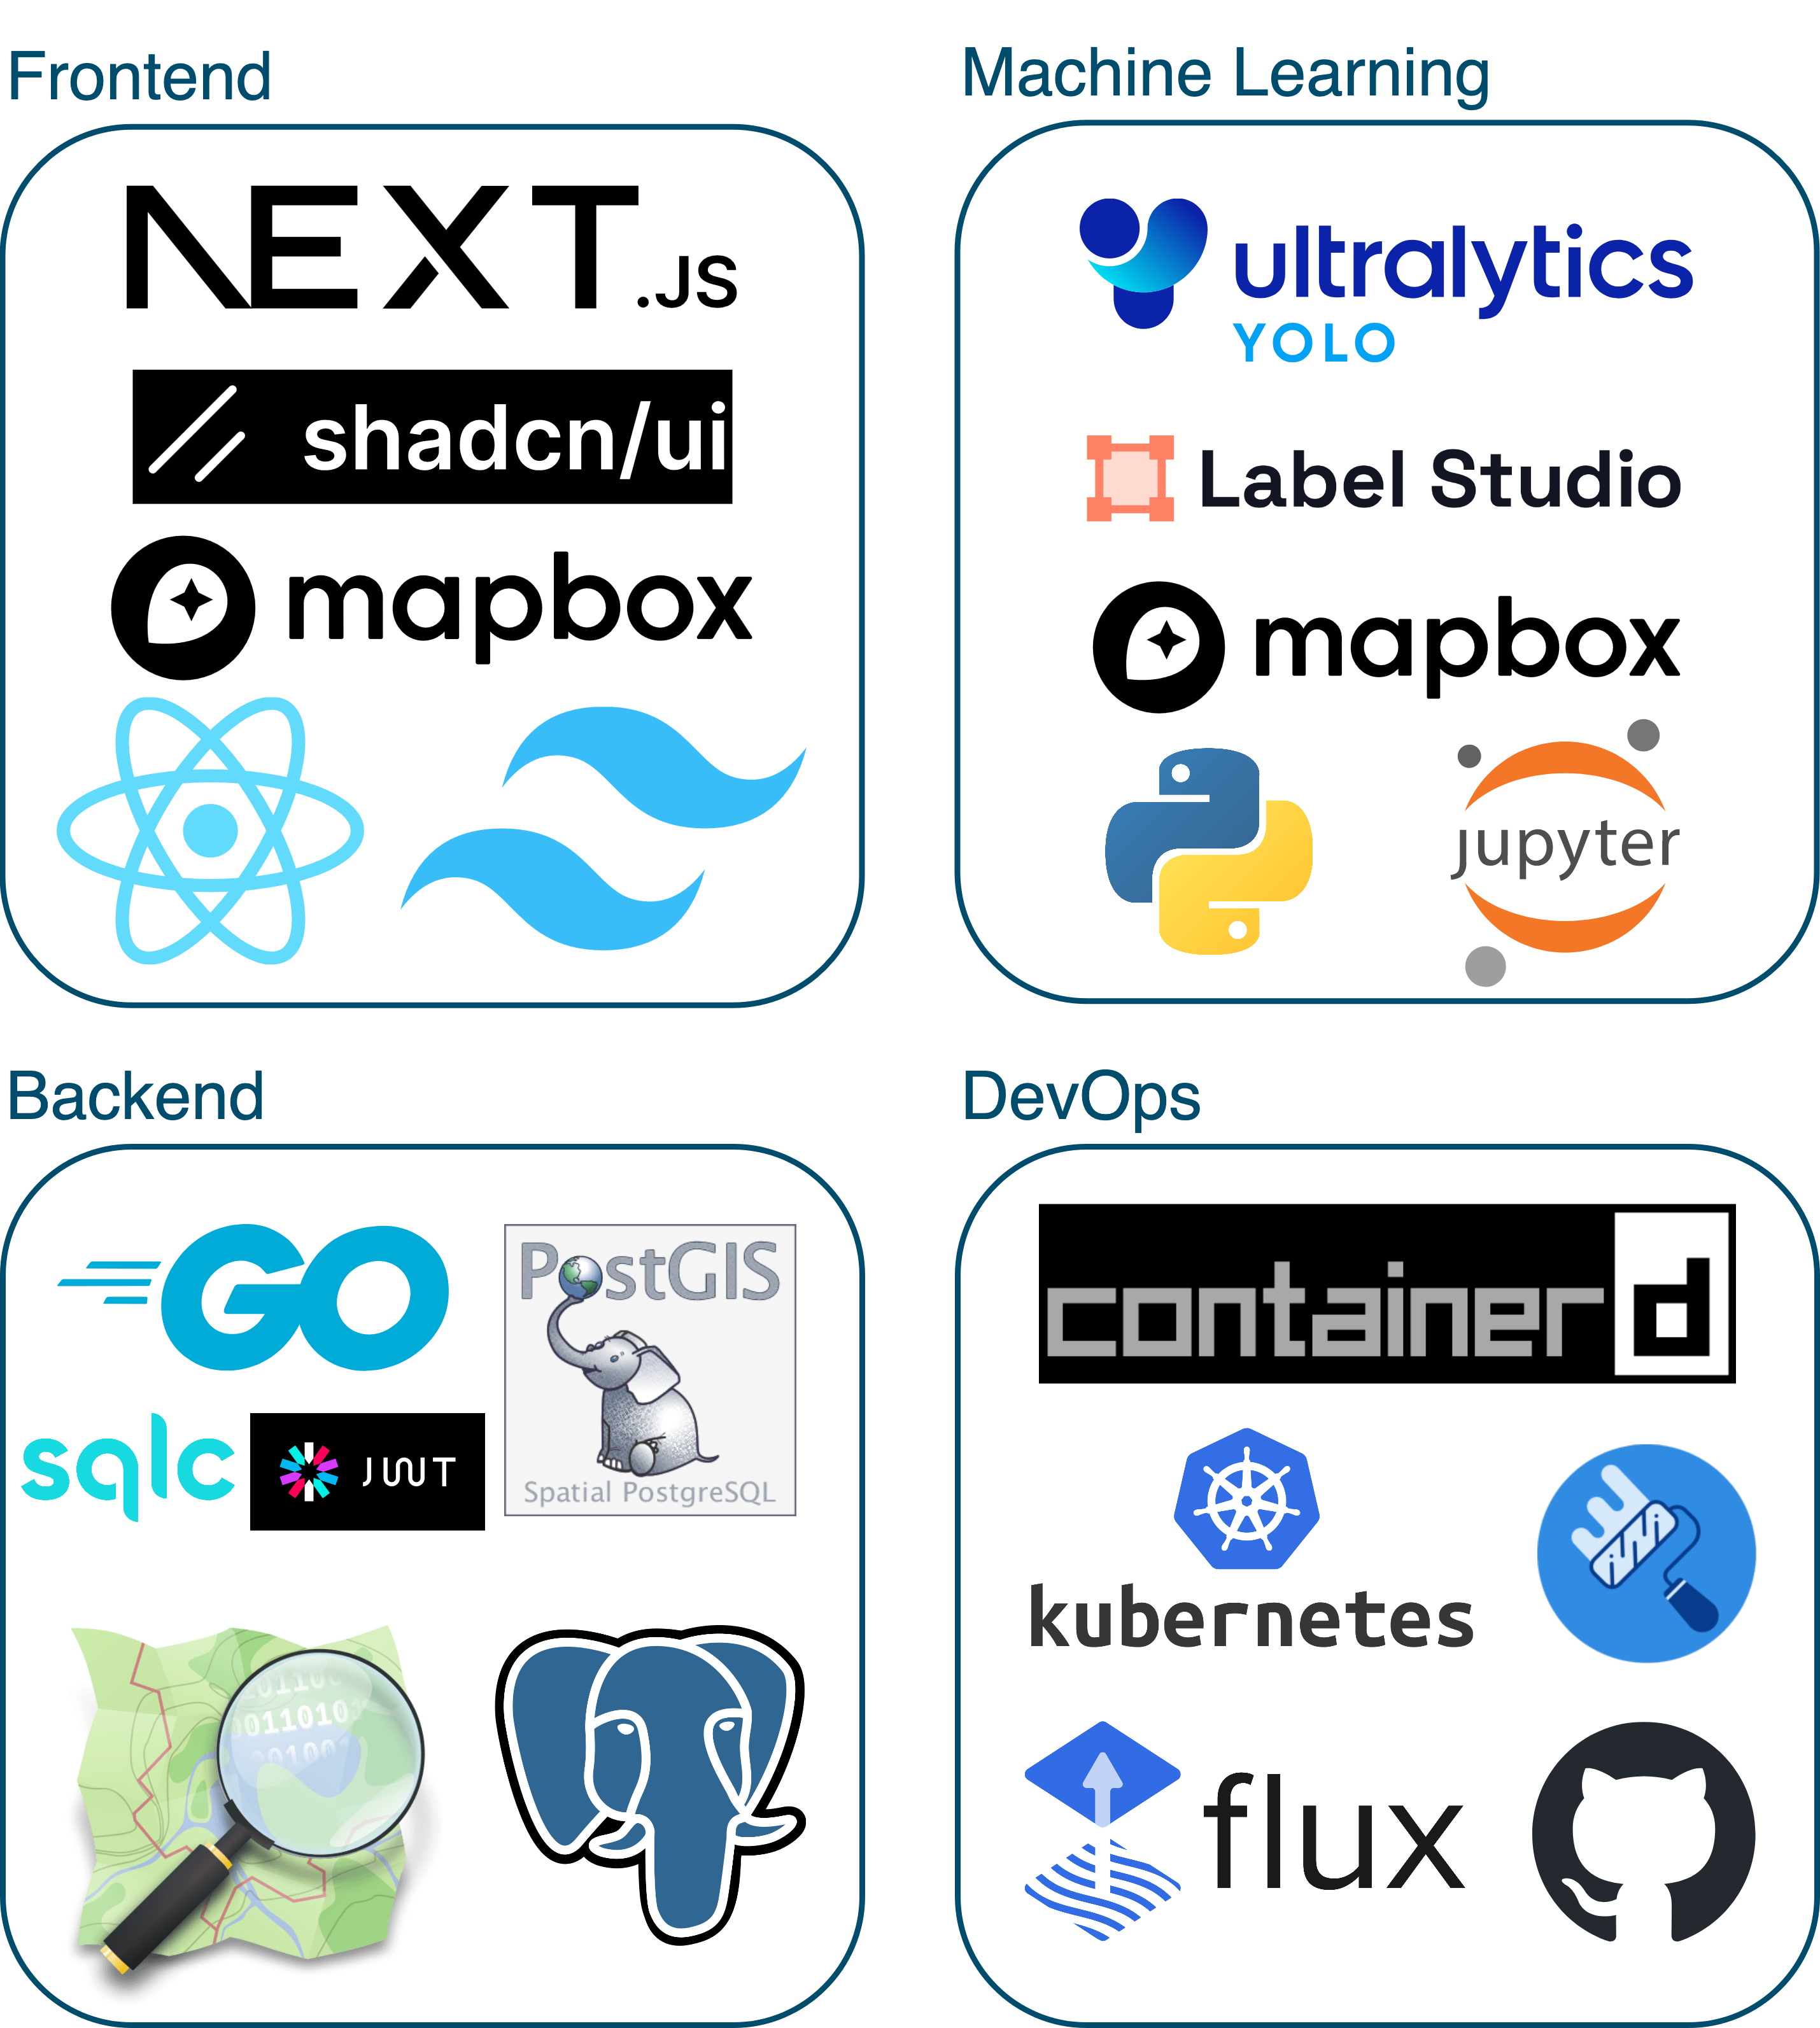
\includegraphics[width=0.5\textwidth]{images/stack_grid.png}
    \caption{Magpie's technology Stack}
\end{figure}

\subsubsection{Frontend Technologies}

The frontend stack plays a critical role in providing a smooth and interactive user experience for the application. It is built on top of modern web technologies, each serving a unique purpose:

\begin{itemize}
    \item{} \textbf{Next.js:} This React framework offers server{-}side rendering (SSR) and static site generation (SSG), which improve performance, SEO, and user experience.
    \item{} \textbf{React:} As the foundation of the frontend, React allows for component{-}based development, making the interface scalable and easy to maintain.
    \item{} \textbf{TailwindCSS:} A utility{-}first CSS framework that simplifies styling by providing ready{-}to{-}use classes, enabling rapid UI development.
    \item{} \textbf{shadcn/ui:} A collection of reusable UI components that work seamlessly with Next.js and React, enhancing productivity and consistency across the application.
    \item{} \textbf{Mapbox:} A powerful mapping platform that enables interactive, customizable maps. It helps visualize geospatial data effectively, which is key for location{-}based services in this project.
\end{itemize}

These technologies combine to create an engaging user interface that is both functional and visually appealing, allowing users to interact with location{-}based data and services efficiently.

\subsubsection{Machine Learning Technologies}

The machine learning stack adds intelligent capabilities to the system, enabling advanced features such as object detection and data annotation. Here’s a breakdown of the tools in this section:

\begin{itemize}
    \item{} \textbf{Ultralytics YOLO:} A real{-}time object detection model that helps identify specific objects in images or maps, enhancing the system's ability to recognize and interpret visual data.
    \item{} \textbf{Label Studio:} A flexible tool for annotating datasets, enabling easy labeling of images, text, and audio. This is crucial for creating high{-}quality datasets to train machine learning models like YOLO\@.
    \item{} \textbf{Python:} The primary language for developing and running machine learning models, Python supports data processing, model training, and analysis.
    \item{} \textbf{Jupyter Notebooks:} An interactive platform that allows data scientists to experiment with code, visualize results, and document their machine learning processes.
\end{itemize}

These technologies allow the application to process and analyze data intelligently, enabling features such as object recognition in geographical data and personalized insights.